%%%%%%%%%%%%%%%%%%%%%%%%%%%%%%%%%%%%%%%%%%%%%%%%%%%%%%%%%%%%%%%%%%%%%%%%%%
%%LaTeX template for papers && theses									%%
%%Done by the incredible ||Z01db3rg||									%%
%%Under the do what ever you want license								%%
%%%%%%%%%%%%%%%%%%%%%%%%%%%%%%%%%%%%%%%%%%%%%%%%%%%%%%%%%%%%%%%%%%%%%%%%%% 

%start preamble
\documentclass[paper=a4,fontsize=11pt]{scrartcl}%kind of doc, font size, paper size
\usepackage[ngerman]{babel}%for special german letters etc			
%\usepackage{t1enc} obsolete, but some day we go back in time and could use this again
\usepackage[T1]{fontenc}%same as t1enc but better						
\usepackage[utf8]{inputenc}%utf-8 encoding, other systems could use others encoding
%\usepackage[latin9]{inputenc}			
\usepackage{amsmath}%get math done
\usepackage{amsthm}%get theorems and proofs done
\usepackage{graphicx}%get pictures & graphics done
\graphicspath{{pictures/}}%folder to stash all kind of pictures etc
\usepackage{amssymb}%symbolics for math
\usepackage{amsfonts}%extra fonts
\usepackage []{natbib}%citation style
\usepackage{caption}%captions under everything
\usepackage{listings}
\usepackage[titletoc]{appendix}
\numberwithin{equation}{section} 
\usepackage[printonlyused,withpage]{acronym}%how to handle acronyms
\usepackage{float}%for garphics and how to let them floating around in the doc
\usepackage{cclicenses}%license!
\usepackage{xcolor}%nicer colors, here used for links
\usepackage{wrapfig}%making graphics floated by text and not done by minipage
\usepackage{dsfont}
\usepackage{stmaryrd}
\usepackage{geometry}
\usepackage{hyperref}
\usepackage{fancyhdr}
\usepackage{menukeys}
\usepackage{multicol}

%settings colors for links
\hypersetup{
    colorlinks,
    linkcolor={blue!50!black},
    citecolor={blue},
    urlcolor={blue!80!black}
}

\definecolor{pblue}{rgb}{0.13,0.13,1}
\definecolor{pgreen}{rgb}{0,0.5,0}
\definecolor{pred}{rgb}{0.9,0,0}
\definecolor{pgrey}{rgb}{0.46,0.45,0.48}

\pagestyle{fancy}
\lhead{Benjamin Tröster\\Netzwerke Übung (Wise2018/19)}
\rhead{FB 4 -- Angewandte Informatik\\ HTW-Berlin}
\lfoot{Übungsblatt 3 -- Routing}
\cfoot{}
\fancyfoot[R]{\thepage}
\renewcommand{\headrulewidth}{0.4pt}
\renewcommand{\footrulewidth}{0.4pt}


\lstdefinestyle{Bash}{
  language=bash,
  showstringspaces=false,
  basicstyle=\small\sffamily,
  numbers=left,
  numberstyle=\tiny,
  numbersep=5pt,
  frame=trlb,
  columns=fullflexible,
  backgroundcolor=\color{gray!20},
  linewidth=0.9\linewidth,
  %xleftmargin=0.5\linewidth
  upquote=true,
  columns=fullflexible,
  literate={*}{{\char42}}1
         {-}{{\char45}}1
}

\newlength\labelwd
\settowidth\labelwd{\bfseries viii.)}
\usepackage{tasks}
\settasks{counter-format =tsk[a].), label-format=\bfseries, label-offset=3em, label-align=right, label-width
=\labelwd, before-skip =\smallskipamount, after-item-skip=0pt}
\usepackage[inline]{enumitem}
\setlist[enumerate]{% (
labelindent = 0pt, leftmargin=*, itemsep=12pt, label={\textbf{\arabic*.)}}}

\pdfpkresolution=2400%higher resolution

%%here begins the actual document%%
\newcommand{\horrule}[1]{\rule{\linewidth}{#1}} % Create horizontal rule command with 1 argument of height

\DeclareMathOperator{\id}{id}

\begin{document}
\begin{center}
\Large{\textbf{Übungsblatt 03 -- Routing}}
\end{center}
\textbf{Hilfreiche Programme:}
\begin{multicols}{3}
\begin{itemize}
	\item ifconfig, ip addr
	\item ip link
	\item route/ip route
	\item sysctl
	\item netstat 
	\item ping
\end{itemize}
\end{multicols}
	
\begin{center}\Large{\textbf{Aufgabe A -- Umsetzung des Routings}}\end{center}\vskip0.25in
%\setlist[enumerate, 1]{itemsep=\baselineskip}
Setzen Sie das aus der Planung hervorgegangene Netzwerk (bzw. die Netzwerke) mit den Ihn bekannten Tools um.
\begin{enumerate}
	\item \textbf{Für die Hosts:}\\
	\begin{tasks}(1)
		\task~ Beschriften Sie die aus den Hausaufgaben hervorgegangene Skizze mit den in der Gruppe zu vergebenen IP-Adressen.\\
		S. Abb. \ref{example_lan}
		\task~ Setzen Sie die IP-Adressen und Routen mithilfe der Kommandos \emph{ip add} und \emph{ip route [add|delete|replace]} aus dem \emph{iproute2}-Werkzeugkasten bzw. den Networking-Tools \emph{ifconfig} und \emph{route add}.  Achten Sie darauf, ob Sie ein Default-Gateway definieren oder ein \glqq herkömmliches\grqq\ Gateway! Beides ist möglich, jedoch erweitern Sie bald Ihr Netzwerk, wodurch sich dies ändern könnte.\\
		\textbf{Antwort:}\\
		\textbf{LAN A:}\\
		\textit{ip addr add 10.0.1.2/29 dev eth0} bzw. \textit{ifconfig eth0 10.1.1.2 netmask 255.255.255.248 up} bzw. \textit{ifconfig eth0 10.1.1.2/29 up}\\
		\textit{ip addr add 10.0.1.3/29 dev eth0} bzw. \textit{ifconfig eth0 10.1.1.3 netmask 255.255.255.248 up}\\
		\textit{ip addr add 10.0.1.1/29 dev eth0} bzw. \textit{ifconfig eth0:0 10.1.1.1 netmask 255.255.255.248 up}\\
		\textbf{LAN B:}\\
		\textit{ip addr add 10.0.2.2/30 dev eth0} bzw. \textit{ifconfig eth0 10.1.2.2 netmask 255.255.255.250 up} bzw. \textit{ifconfig eth0 10.1.2.2/30 up}\\
		\textit{ip addr add 10.0.2.1/29 dev eth0} bzw. \textit{ifconfig eth0:1 10.1.2.1 netmask 255.255.255.250 up}\\
		\textbf{Routen:}\\
		Von LAN A nach LAN B\\
		\textit{ip route add 10.0.2.0/30 via 10.0.1.1 dev eth0} bzw. \textit{route add -net 10.0.2.0 netmask 255.255.255.250 gw 10.0.1.1}\\
		Von LAN B nach LAN A\\
		\textit{ip route add 10.0.1.0/29 via 10.0.2.1 dev eth0} bzw. \textit{route add -net 10.0.1.0 netmask 255.255.255.248 gw 10.0.2.1}
		\task~ Nachdem Sie die Routen entsprechend Ihrer Planung eingetragen haben, sollten Sie schauen, wie die Routing-Tabelle aussieht. Analysieren Sie die Ihnen vorliegende Routing-Tabelle. Was bedeuten die Einträge? Bzw. entspricht die Ausgabe Ihren Erwartungen?\\
	\textbf{Antwort:}\\
	Da der Router beide Netzwerke kennt sind im Routing-Table nur diese beiden Einträge zu sehen. Die Hosts haben jeweils einen Eintrag mit dem Zielnetwerk und dem anzusprechenden Gateway.\\
	\textbf{Router:}\\
	10.0.1.0/29 dev eth0 proto kernel scope link src 10.0.1.1 metric 100\\
	10.0.2.0/30 dev eth0 proto kernel scope link src 10.0.2.1 metric 100\\
	\textbf{Hosts:}\\
	10.0.2.0/30 via 10.0.1.1 dev eth0 proto static metric 100 
	\end{tasks}
	\begin{figure}[H]
		\center
		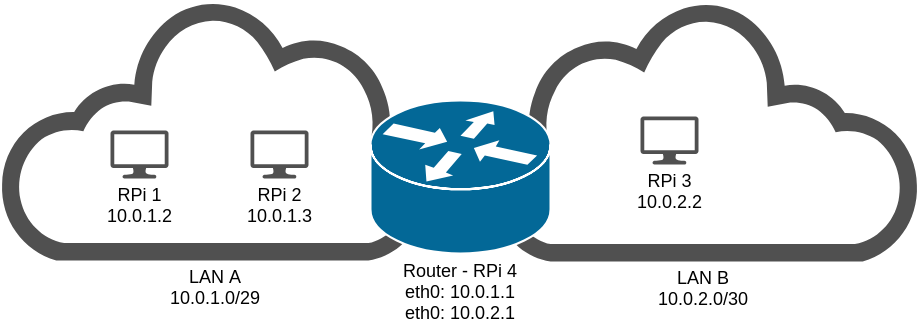
\includegraphics[scale=0.3]{example_lan}
		\caption{Beispielnetzwerk für ein einfach LAN mit zwei Segmenten A und B, sowie einem Router. Der Router ist in beiden Netzwerken Teilnehmer und dient als vermittelnder Zwischenknoten.}
		\label{example_lan}
		\end{figure}
	\item \textbf{Für den Router:}\\
	Der Router benötigt eine etwas andere Konfiguration. 
	\begin{tasks}(1)
		\task~ Konfigurieren Sie am Router die IP-Adressen des Netzwerkadapters. Wenn Ihr Router zwischen zwei Netzwerken vermittelt, sollte dieser beide Netzwerke kennen. D.h. Ihr Router ist Teilnehmer an beiden Netzwerken und benötigt zwei IP-Adressen, für jedes Netzwerk eine.\\
		S. oben!
		\task~ Nachdem der Router konfiguriert wurde, sollten die Raspberry Pis aus den beiden Netzen versuchen diesen via Ping zu erreichen.\\
		\textbf{Antwort:}\\
		Bspw.: \textit{ping -c1 10.0.2.2} 
		\task~ Testen Sie welche der anderen IP-Adressen Sie nun anpingen können und welche nicht.\\
		\textbf{Antwort:}\\
		Nur die Hosts innerhalb eines Netzwerks bzw. der Router beide Netzwerke, da dieser Teilnehmer in beiden Netzwerken ist.
		\end{tasks}
		\item Sie können mithilfe eines kleine Chats testen, ob Pakete tatsächlich auf dem Router ankommen. Dafür basteln Sie eine kleine  Client-Server-Lösung. Beide Seiten nutzen das Tool \emph{netcat -- nc}. Das Listing \ref{netcat_server} zeigt die Seite des Servers, dieser Stellt den \glqq Server\grqq\ bereit, der Client darf sich anschließen mithilfe eines \emph{Sockets (Tupel aus IP-Adresse und Port)} verbinden (s. Listing \ref{netcat_client}). 
		\item \textbf{Alternativ:} Wenn Sie bereits mit Wireshark gearbeitet haben können Sie auch dies benutzen, um festzustellen, ob die Pakete korrekt ankommen.\\
		
	\begin{lstlisting}[style=Bash, language=Bash, label={netcat_server}]
#Server port > 1024 
nc -l -p <port_number> <ip_of_server>
#example
nc -l -p 4711 10.0.0.1
		\end{lstlisting}
		
		\begin{lstlisting}[style=Bash, language=Bash, label={netcat_client}]
#Client 
nc <ip_of_server> <port_number>
#example
nc 10.0.0.1 4711
		\end{lstlisting}
	\item \textbf{Router: Forwarding}\\
	Im Idealfall sollten Sie den Router auf beiden IP-Adressen erreichen können -- andere Rechner außerhalb ihres Netzes antworten Ihnen nicht (Sie können dies ruhig austesten!). Das Weiterleiten von Paketen muss auf dem Router explizit erlaubt werden, dies hat Sicherheitsgründe -- ansonsten könnten Pakete von Fremden im Netz beliebig versendet werden (Bspw.: Wenn Sie in Ihrem Notebook neben ihrem WiFi noch eine WWAN-Karte für teure LTE-Verbindugen betreiben, könnten andere Teilnehmer \glqq kostengünstig\grqq\ mitsurfen.)
	\begin{tasks}(1)
		\task~ Schauen Sie sich die Routing-Tabelle auf dem Router an. Welche Informationen können Sie diesem entnehmen?\\
		\textbf{Antwort:}\\
		Der Router ist Teilnehmer beider Netzwerke und kann entsprechend Pakete in beide Zielnetzwerke schicken, da er alle Hosts direkt ermitteln kann.
        \task~ Muss am Router eine Anpassung der Routing-Tabelle vorgenommen werden, so das dieser weiß wohin er die Pakete senden muss?\\
        \textbf{Antwort:}\\
        Nein! Der Router kennte beide Netzwerke, dies ist für den hier abzuarbeitenden Fall ausreichend.
        \task~ Aktivieren Sie das Forwarding im Betriebssystem des Routers, sodass ein Routing möglich ist. Ihre Umsetzung \textbf{muss} eine nicht persistente Lösung sein! D.h. es soll in keine Datei geschrieben werden.\\
        \textbf{Antwort:}\\
        \textit{sysctl net.ipv4.ip\_forward} bzw. \textit{sysctl -w net.ipv4.ip\_forward}
		\task~ Testen Sie jeweils mit einem \glqq ping\grqq\ aller beteiligten Rechner, welche Netzwerke und IP-Adressen Sie erreichen können und welche nicht.
		\task~ Notieren Sie sich auftretende Fehlermeldungen und vergleichen Sie deren Ursache mit Ihren Recherchen aus den Hausaufgaben.
		\task~ Nutzen Sie erneut den Chat-Server mit \emph{netcat} um zu überprüfen, ob Ihr Netzwerk korrekt funktioniert. D.h. zwei Hosts aus unterschiedlichen Teilen Ihres Netzwerkes sollen miteinander kommunizieren.
	\end{tasks}
\item \textbf{Sofern Sie keine eigene SD-Karte nutzen:} Setzen Sie die Einstellungen des Raspberry Pis bzw. des Betriebssystems zurück die Sie vorgenommen haben! D.h. setzen Sie das Betriebssystem auf den initialen Zustand samt \emph{dhcp} zurück. Haken Sie zumindest folgende Liste ab:
\begin{itemize}
	\item Eigene IP-Config zurücksetzen:
	\begin{itemize}
		\item \path{/etc/network/interfaces}
		\item Bash-Script: \emph{reset\_network\_config.sh}
	\end{itemize}
	\item Routing/Forwarding:
	\begin{itemize}
		\item Keine persistenten Routen vorhanden?
		\item Forwarding deaktiviert? 
		\item \path{/etc/systctl.conf}
		\item \path{/proc/sys/net/ipv4/ip_forward}
	\end{itemize}
	\item DNS
	\begin{itemize}
		\item DNS Einträge verändert?
		\item \path{/etc/resolv.conf}
		\item \emph{reset\_hosts.sh}
	\end{itemize}
	\item DHCPcd:
	\begin{itemize}
		\item \emph{sudo systemctl enable dhcpcd}
		\item \emph{nw\_default.sh}
	\end{itemize}
\end{itemize}
\end{enumerate}
\end{document}